%----------------------------------------------------------------------------------------
%	PACKAGES AND THEMES
%----------------------------------------------------------------------------------------
\documentclass[aspectratio=169,xcolor=dvipsnames]{beamer}
\usetheme{SimplePlusAIC}
\usepackage{comment}
\usepackage{hyperref}
\usepackage{csquotes}
\newcommand{\code}[1]{\texttt{#1}}
\usepackage{graphicx} % Allows including images
\usepackage{booktabs} % Allows the use of \toprule, \midrule and  \bottomrule in tables
\usepackage{svg} %allows using svg figures
\usepackage{tikz}
\usepackage{makecell}
\newcommand*{\defeq}{\stackrel{\text{def}}{=}}

%Select the Epilogue font (requires luaLatex or XeLaTex compilers)
\usepackage{fontspec}
\usepackage{listings}
\usepackage{matlab-prettifier}

% Define MATLAB code style
\lstset{
  style=Matlab-editor,
  basicstyle=\ttfamily\scriptsize,
  frame=single,
  numbers=left,
  numberstyle=\tiny,
  breaklines=true,
}


\setsansfont{Epilogue}[
    Path=./epilogueFont/,
    Scale=0.9,
    Extension = .ttf,
    UprightFont=*-Regular,
    BoldFont=*-Bold,
    ItalicFont=*-Italic,
    BoldItalicFont=*-BoldItalic
    ]

%----------------------------------------------------------------------------------------
%	TITLE PAGE
%----------------------------------------------------------------------------------------

\title[SVD \& Its Appl.]{Low Rank Singular Value Decomposition and Its Application} % The short title appears at the bottom of every slide, the full title is only on the title page

\author[Ivan L. Ihwani]{Ivan L. Ihwani}
\institute[M115 2024]{Department of Mathematics \newline National Central University}
% Your institution as it will appear on the bottom of every slide, maybe shorthand to save space


\date{July 3, 2024} % Date, can be changed to a custom date
%----------------------------------------------------------------------------------------
%	PRESENTATION SLIDES
%----------------------------------------------------------------------------------------

\begin{document}

\begin{frame}[plain]
    % Print the title page as the first slide
    \titlepage
\end{frame}

\begin{frame}{Overview}
    % Throughout your presentation, if you choose to use \section{} and \subsection{} commands, these will automatically be printed on this slide as an overview of your presentation
    \tableofcontents
\end{frame}

%------------------------------------------------
\section{Motivation}
\begin{frame}{Motivation}
Why we want to do this?
\begin{enumerate}
\item \textit{De-noising:} If a matrix $A$ is a noisy version of some \enquote{ground truth} signal, then a low-rank approximation of the raw data $A$ might throw out lots of noise and little signal, resulting in a matrix that is more informative than the original.
\item \textit{Dimensionality Reduction:} Compressing data into a lower-dimensional representation reduces computational costs and storage requirements.
\item \textit{Feature Extraction:} Identifying the most prominent features within a dataset can enhance analysis and modeling.
\item \textit{Updating Huge ML Models:} One quite modern application of low-rank matrix approximations is for \enquote{fine-tuning} huge models. \textbf{See} the paper of \textcolor{blue}{LORA: Low-Rank Adaptation of Large Language Models}.
\end{enumerate}
\end{frame}

\section{What is SVD?}
%------------------------------------------------
\begin{frame}{What is SVD?}
The SVD factorization of $A$ is $A=U\Sigma V^{T}$ where:
\begin{itemize}
    \item $U$ is $m\times m$, $U^{T} U=I_{m}$, 
    \item $V$ is $n\times n$, $V^{T} V = I_{n}$,
    \item $\Sigma$ is $m\times n$ where $\Sigma = \begin{bmatrix}
        \Sigma_{r} & 0_{r\times (n-r)}\\
        0_{(m-r)\times r} & 0_{(m-r)\times (n-r)}
    \end{bmatrix}$, and
    \item $\Sigma_r = \begin{bmatrix}
        \sigma_1 & & \\
         & \ddots & \\
          & & \sigma_r 
    \end{bmatrix}$ with $\sigma_1 \geq \dots \geq \sigma_r \geq 0 $.
\end{itemize}

\textbf{remark:} $U \neq V$ and $\text{size}(U) \neq \text{size}(V)$.
\end{frame}

%------------------------------------------------
\section{Low Rank SVD}
\begin{frame}{Low-Rank Approximations with SVD}
\begin{itemize}
    \item If we want to best approximate a matrix $A$ by a rank-$k$ matrix, how should we do it?
    \item If only we has a representation of the data matrix $A$ as a sum of several ingredients, with these ingredients ordered by \enquote{importance,} then we could just keep the $k$ \enquote{most important} ones. \item The SVD gives exactly such a representation!.
    \begin{equation}
        \label{eq:1}
        \hat{A} = \sum^{k}_{i=1} \sigma_{i} \cdot \textbf{u}_i \textbf{v}^{T}_i .
    \end{equation}
  \end{itemize}
\end{frame}

\begin{frame}{Low-Rank Approximations with SVD}
An equivalent way to think about the proposed rank-$k$ approximation:
\begin{enumerate}
    \item Compute the SVD $A=USV^{T}$, where $U$ ia an $m\times m$ orthogonal matrix, $S$ is a nonnegative $m\times n$ diagonal matrix with diagonal entries sorted from high to low, and $V^{T}$ is a $n\times n$ orthogonal matrix. 
    \item Keep only the top $k$ right singular vectors: set $V^{T}_k$ equal to the first $k$ rows of $V^{T}$ (a $k\times n$ matrix).
    \item Keep only the top $k$ left singular vectors: set $U_{k}$ equal to the first $k$ columns of $U$ (an $m\times k$ matrix).
    \item Keep only the top $k$ singular values: set $\Sigma_{k}$ equal to the first $k$ rows and columns of $\Sigma$ (a $k\times k$ matrix), corresponding to the $k$ largest singular values of $A$.
    \item The rank-$k$ approximation is then 
    \begin{equation}
    \label{eq:2}
        A_{k} = U_k \Sigma_k V^{T}_{k} .
    \end{equation}
\end{enumerate}
\end{frame}

%------------------------------------------------

\begin{frame}{Low-Rank Approximations with SVD}
    Storing the matrices on the RHS of \eqref{eq:2} takes $\mathcal{O}(k(m+n))$ space, in contrast to the $\mathcal{O}(mn)$ space required to store tha original matrix $A$. This is a \textbf{big win} when $k$ is small relative to $m$ and $n$.
    \begin{figure}[H]
    \centering
    \includegraphics[width=7cm]{images/SVDk.jpg}
    \caption{Low rank approximation via SVD. Recall that $\Sigma$ is non-zero only on its diagonal, and the diagonal entries of $\Sigma$ are sorted from high to low.}
    \label{Fig1}
\end{figure}
\end{frame}

%------------------------------------------------------------------------
\begin{frame}{Example 1}
$A = \begin{bmatrix}
    1 & 1\\ 2 & 2
\end{bmatrix}$, where $n=m=2$ and rank$(A)=1$.\\
$A^{T} A = \begin{bmatrix}
    5 & 5\\ 5 & 5
\end{bmatrix}$ and det$\left( \begin{bmatrix}
    5-\lambda & 5\\ 5 & 5-\lambda
\end{bmatrix}\right) = 0$ implies $\lambda_1=10$, $\sigma_1=\sqrt{10}$, and $\lambda_2=0$, $\sigma_2 =0$.\\
The first eigenvectors are
\begin{align*}
    \textbf{v}_1 &= \begin{bmatrix}
        1 / \sqrt{2}\\
        1/\sqrt{2}
    \end{bmatrix}\, \quad\text{and}\\
    \textbf{u}_1 &= \frac{A \textbf{v}_1}{\sigma_1} = \begin{bmatrix}
        1 / \sqrt{5} \\ 2 / \sqrt{5}
    \end{bmatrix} .
\end{align*}
This gives a \enquote{small} (or rank-1 SVD) 
\begin{align*}
    \textbf{u}_1 \sigma_1 \textbf{v}^{T}_1 = \begin{bmatrix}
        1 / \sqrt{5} \\ 2 / \sqrt{5} 
    \end{bmatrix} \sqrt{10} \begin{bmatrix}
        1 / \sqrt{2} & 1/ \sqrt{2}
    \end{bmatrix} = \begin{bmatrix}
        1 & 1\\ 2 & 2
    \end{bmatrix} .
\end{align*}
\end{frame}

\begin{frame}{Example 1 (Continuation)}
    The \enquote{full} SVD uses the $\textbf{v}_2$ basis for $N (A)$: $\textbf{v}_2 = \begin{bmatrix}
        1 / \sqrt{2} \\ -1 / \sqrt{2}
    \end{bmatrix}$ and the $\textbf{u}_2$ basis for $N(A^{T})$: $\textbf{u}_2 = \begin{bmatrix}
        -2 / \sqrt{5}\\ 1/ \sqrt{5} 
    \end{bmatrix}$.\\
    \begin{align*}
        U \Sigma V^{T} &= \begin{bmatrix}
            \textbf{u}_1 & \textbf{u}_2
        \end{bmatrix} \begin{bmatrix}
            \sigma_1 & 0\\
            0 & 0
        \end{bmatrix} \begin{bmatrix}
            \textbf{v}^{T}_1 \\ \textbf{v}^T_2
        \end{bmatrix} \\
        &= \begin{bmatrix}
            1/\sqrt{5} & -2/\sqrt{5} \\
            2/ \sqrt{5} & 1/\sqrt{5}
        \end{bmatrix} \begin{bmatrix}
            \sqrt{10} & 0\\
            0 & 0
        \end{bmatrix} \begin{bmatrix}
            1/ \sqrt{2} & 1/ \sqrt{2}\\
            1/ \sqrt{2} & -1/\sqrt{2}
        \end{bmatrix}\\
        &= \begin{bmatrix}
            1 & 1\\ 2 & 2
        \end{bmatrix}.
    \end{align*}
\end{frame}

\begin{frame}{Fact}
 %   This low-rank approximation is \textit{optimal} in a natural sense. The guarantee is in terms of the \enquote{Frobenius norm} of a matrix $M$, i.e. applying the $\ell_2$ norm to the matrix as if it were a vector: $\left\| M \right\|_F = \sqrt{\sum_{i,j} m^2_{ij}}$.\\
%    \vspace{1cm}
    For every $m\times n$ matrix $A$, rank target $k\geq 1$, and rank-$k$ $m\times n$ matrix $B$,
    \begin{equation}
        \label{eq:3}
        \left\| A - A_k\right\|_F \leq \left\| A- B\right\|_F ,
    \end{equation}
    where $A_k$ is the rank-$k$ approximation \eqref{eq:2} derived from the SVD of $A$.
\end{frame}

%--------------
\begin{comment}
\begin{frame}{Example 2}
   \begin{figure}[h]
\includegraphics[width=8cm]{images/result1.png}
\end{figure}
\end{frame}

\begin{frame}
   \begin{figure}[h]
\includegraphics[width=7cm]{images/result2.png}
\end{figure}
\end{frame}

\begin{frame}
   \begin{figure}[h]
\includegraphics[width=7cm]{images/result3.png}
\end{figure}
\end{frame}
\end{comment}

% ---------------------------
\begin{frame}{Remark 1: How to Choose $k$}
\begin{itemize}
    \item \textbf{In a perfect world:} if the top few such values are big and the rest are small, then the obvious solution is to take $k$ equal to the number of big values.
    \item \textbf{In a less perfect world:} one takes $k$ as small as possible subject to obtaining a useful approximation.
\end{itemize}
\vspace{1cm}
Rules of thumb: choose $k$ such that the sum of the top $k$ singular values is at least $c$ times as big as the sum of the other singular values, where $c$ is a domain-dependent constant (like
10, say).
\end{frame}

\begin{comment}
\begin{frame}{Remark 2: Lossy Compression via Truncated Decomposition}
Low-rank SVD is another example of a useful paradigm for lossy compression:
   \begin{enumerate}
       \item The 1st step of the paradigm is to re-express the raw data exactly as a decomposition into several terms.
       \item The 2nd step is to throw away all but the \enquote{most important} terms to approximate the representation the raw data.
   \end{enumerate}
   \vspace{1cm}
   Rule of thumb: messy enough data sets might not admit any nice representations at all.
\end{frame}
\end{comment}
% ----------------------------------------------------
\section{Applications}
\begin{frame}[fragile]{Application 1: Image Compression}
\begin{lstlisting}[language=Matlab]
% Load image
img = imread('image.jpg');
img = double(rgb2gray(img)); % Convert to grayscale and double precision

% Compute SVD
[U, S, V] = svd(img);

% Retain only k singular values
k = 50; % You can adjust this value
Uk = U(:, 1:k);
Sk = S(1:k, 1:k);
Vk = V(:, 1:k);

% Reconstruct image
compressed\_img = Uk * Sk * Vk';
\end{lstlisting}
\end{frame}

\begin{frame}{Application 1: Image Compression}
   \begin{figure}[h]
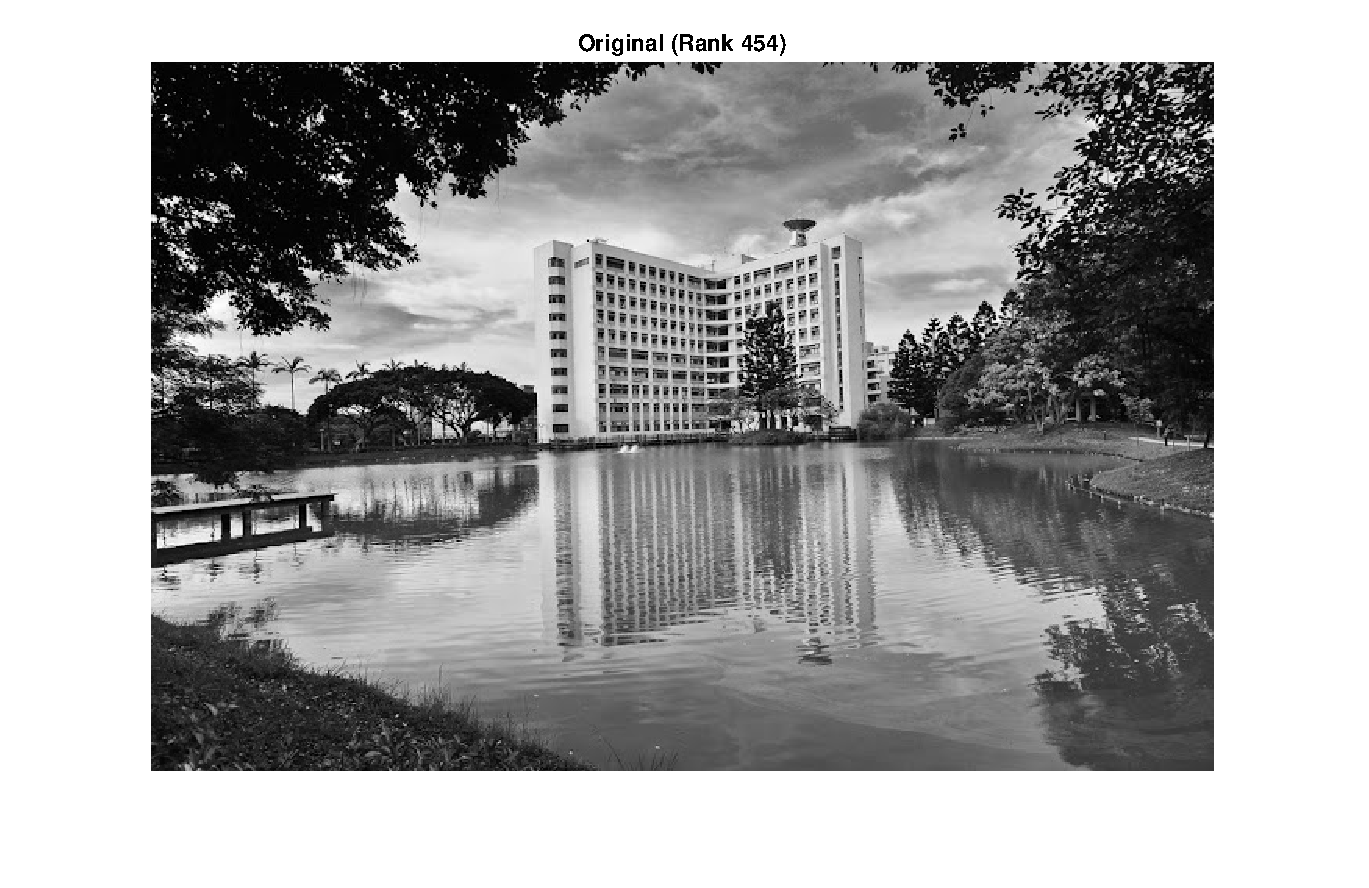
\includegraphics[width=7cm]{images/ori.eps}
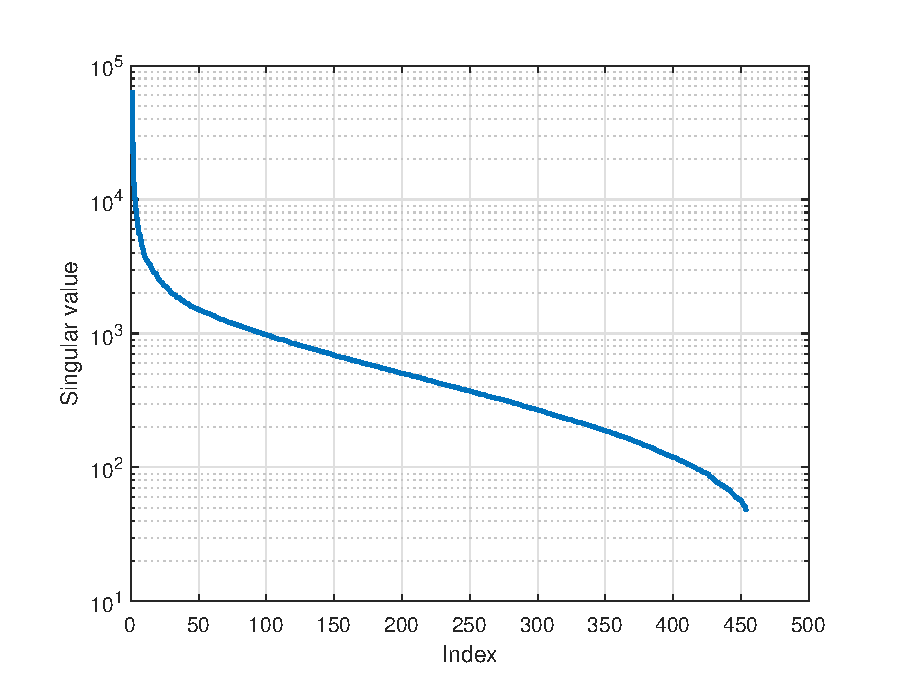
\includegraphics[width=7cm]{images/sv.eps}
\label{Fig2a}
\end{figure}
\end{frame}

\begin{frame}{Application 1: Image Compression}
   \begin{figure}[h]
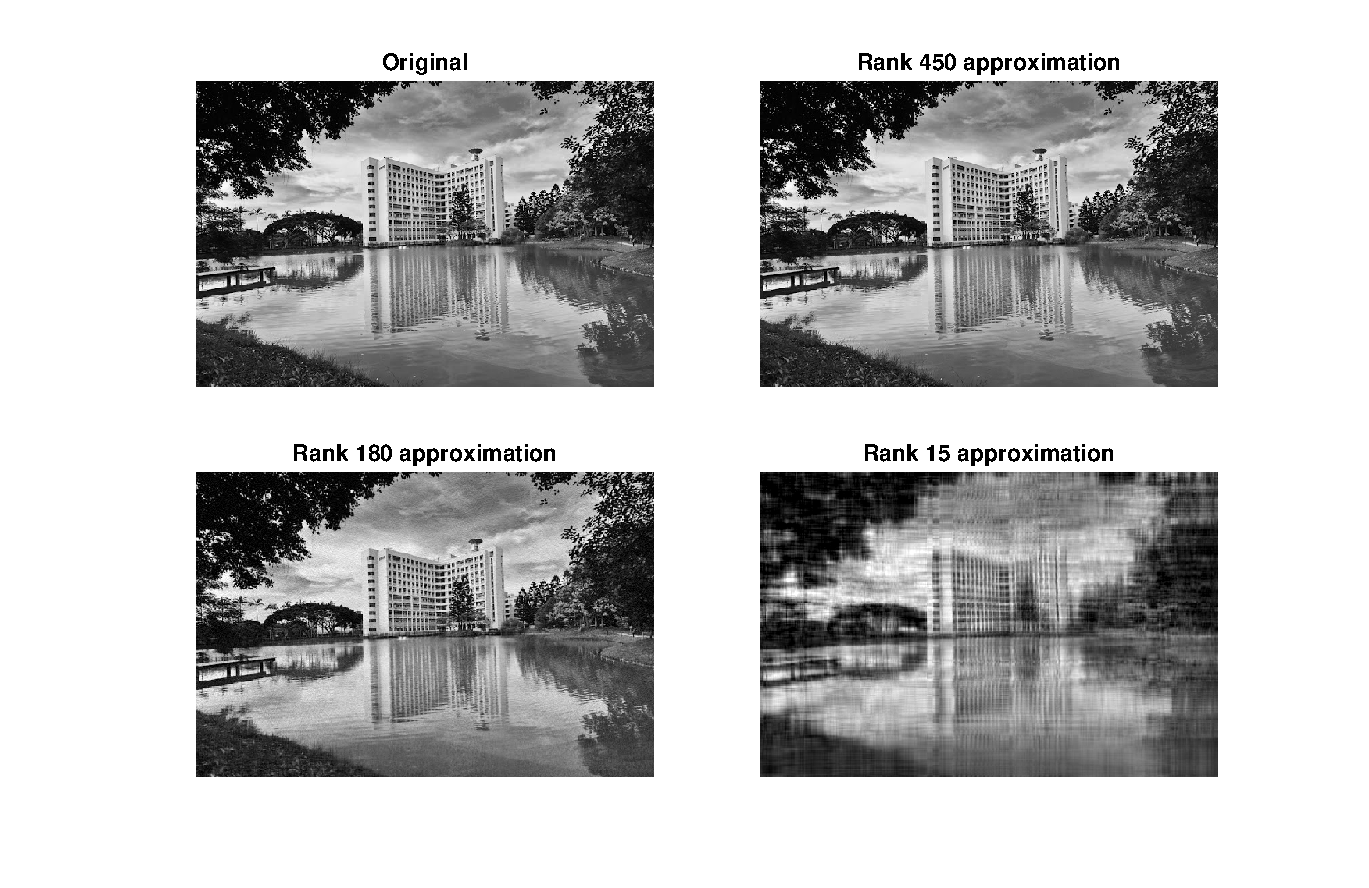
\includegraphics[width=12cm]{images/svdlowrank.eps}
\label{Fig2}
\end{figure}
\end{frame}

%-----------------------------------------------
%------------------------------------------------
\begin{frame}{Application 2: Noise Filter}
 Consider a discrete signal $f
 \in \mathbb{R}^{n}$, some blurring ($K$ an $n\times n$ matrix), and some signal noise ($\eta \in \mathbb{R}^{n}$). The data received ($d\in \mathbb{R}^{n}$) is given by
 \begin{equation}
     d = K f + \eta .
     \label{eq:4}
 \end{equation}
 The objective is to approximate $f$ from the data $d$. \\
 %\textbf{There are two problems:} the noise is not known, and the matrix inversion tends to be sensitive to variations in the data.
 The matrix $K$ has exponential components
 \begin{equation*}
     K = \left[ h Ce^{-((i-j)h)^2 / 2 \gamma^2 }\right] , \quad \text{with} \quad \, h=1/n .
 \end{equation*}
 It is nonsingular, but it has very small singular values, for example, $K$ has $\sigma_n = 4.2275 \times 10^{-7}$.
\end{frame}

\begin{frame}{Application 2: Noise Filter}
    The SVD of $K=U\Sigma_n V^T$ (three $n\times n$ matrices) and $\sigma_i > 0$. Use the orthonormal properties to get
    \begin{align*}
        K^{-1} &= V \Sigma_n^{-1} U^T \quad \text{and}\\
        K^{-1} d &= f + K^{-1} \eta \quad\text{(from \eqref{eq:4})}\\
        V\left( \Sigma^{-1}_n U^T d\right) &= f + V \left( \Sigma^{-1}_n U^{T} \eta \right) .
    \end{align*}
   Since the noise vector $\eta$ has higher frequency components, one can drop some of the latter terms in the SVD, i.e. use the truncated SVD: $K^{(k)} = U^{(k)} \Sigma_k \left( V^{(k)}\right)^T$ with $k< \text{rank}(K) = n$. 
\end{frame}

\begin{frame}{Application 2: Noise Filter}
    The computed signal is
    \begin{align*}
        \hat{f} &= V^{(k)} \left( \Sigma^{-1}_{k} \left( U^{(k)}\right)^T d \right)\\
        &= \sum^{k}_{j=1} v_j \frac{1}{\sigma_j} u^T_j d \\
        &= \sum^{k}_{j=1} \left( \frac{1}{\sigma_j} u^T_{j} d\right) v_j .
    \end{align*}
    Depending in the choice the truncation, the $\sigma_j$ may still be small s.t. variations in the data can cause large errors. 
\end{frame}

\begin{frame}{Application 2: Noise Filter}
    One possible remedy is to replace $\frac{1}{\sigma_j}$ by $\frac{1}{\sigma_j} \frac{\sigma^2_j}{\sigma^2_j + \alpha}$ where $\alpha>0$ (Truncated Tikhonov-Phillips regularization), that is
    \begin{align*}
        \tilde{f} &= \left( \left( K^{(k)}\right)^T K^{(k)} + \alpha I_k\right)^{-1} \left( K^{(k)}\right)^T d\\
        &= \sum^{k}_{j=1} \left( \frac{\sigma_j}{\sigma^2_j + \alpha} u^T_j d \right) v_j .
    \end{align*}
    \textbf{Remark:} The selection of $\alpha > 0$ and $k<n$ can be subjective. 
\end{frame}

\begin{frame}{Application 2: Noise Filter}
    \begin{itemize}
        \item The matrix $K$ is $100\times 100$.
        \item The singular values vary from largest to very very small, i.e. $\sigma_1 = 0.9985$, $\sigma_{40} = 0.0944$, and $\sigma_{100} = 4.2267\times 10^{-7}$.
        \item The eigenvectors $u_j$ and $v_j$ have more oscillations as $j$ increases.
    \end{itemize}
      \begin{figure}[h]
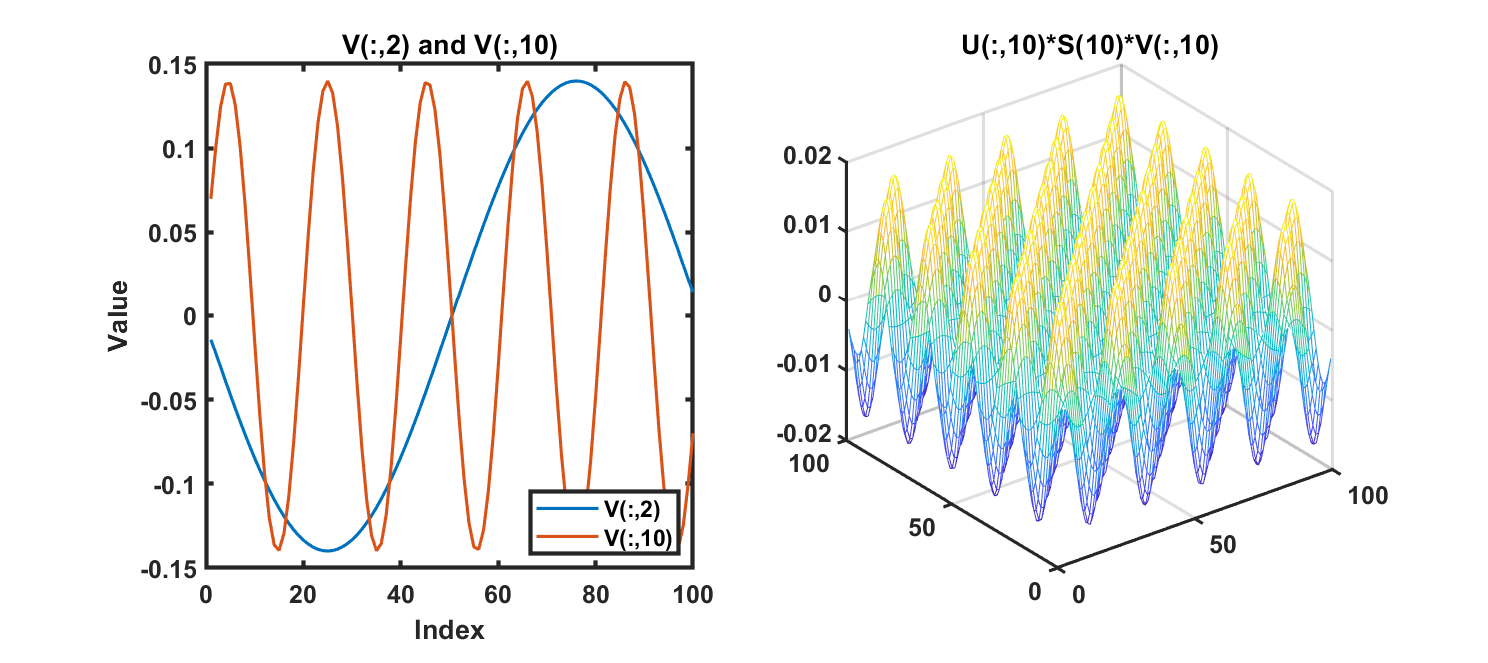
\includegraphics[width=11.5cm]{images/eigenvectors.eps}
\label{Fig3}
\end{figure}
\end{frame}

\begin{frame}{Application 2: Noise Filter}
     \begin{figure}[h]
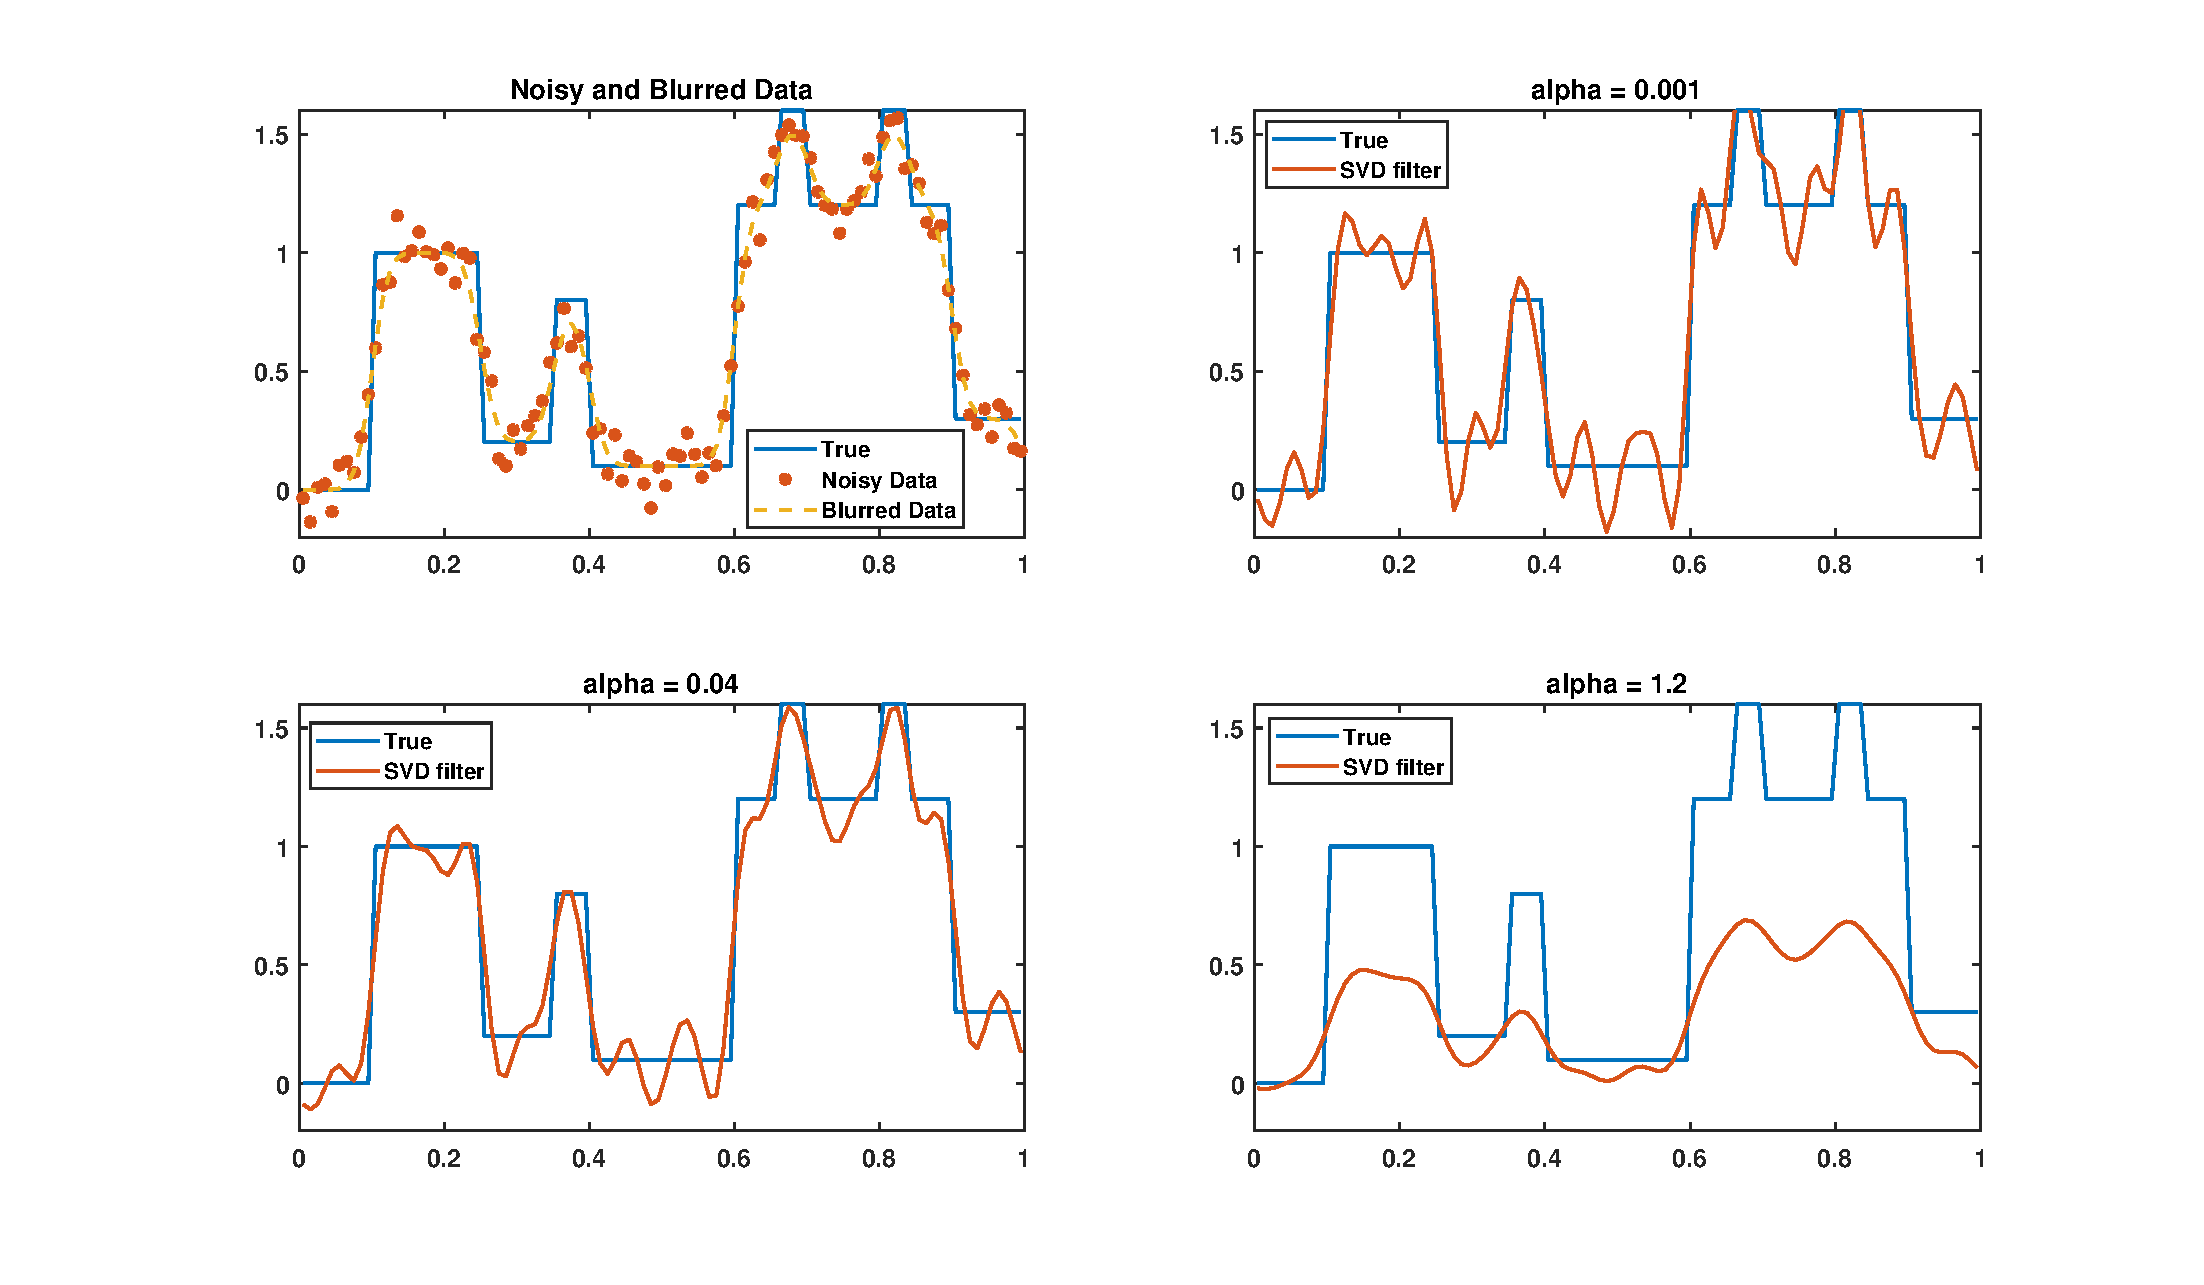
\includegraphics[width=13cm]{images/noisy_and_blurred.eps}
\label{Fig4}
\end{figure}
\end{frame}

\begin{frame}{Other Application}
    \begin{itemize}
        \item Dynamical Low rank approximations for the time dependent PDEs scheme. See \textcolor{blue}{(Koch, O. and Lubich, C., 2007)} and \textcolor{blue}{(Lubich, C. and Oseledets, I. V., 2014)}.
        \item  Implicit step-truncation integration of nonlinear PDEs on low-rank tensor manifolds. See \textcolor{blue}{(Rodgers, A. and Venturi, D., 2022)}.
        \item  Hierarchical adaptive low-rank format with applications
to discretized partial differential equations. See \textcolor{blue}{(Massei, S., Robol, L., and Kressner, D., 2022)}.
\item Implicit low-rank Riemannian schemes for the time
integration of stiff partial differential equations. See \textcolor{blue}{(Sutti, M. and Vandereycken, B., 2023)}.
    \end{itemize}
\end{frame}

\section{Summary}

\begin{frame}{Summary}
  Singular Value Decomposition (SVD) and low-rank approximations provide a powerful set of tools for deriving significant insights from matrices, facilitating data exploration and analysis in a wide range of disciplines.
\end{frame}


%------------------------------------------------
\begin{comment}
\begin{frame}{References}
    % Beamer does not support BibTeX so references must be inserted manually as below
    \footnotesize{
        \begin{thebibliography}{99}
            \bibitem[Agostini A., Markwig, H., Noliau, C., Schleis, V., Sendra-Arranz, J., Sturmfels, B., 2022]{p1} Agostini A., Markwig, H., Noliau, C., Schleis, V., Sendra-Arranz, J., \& Sturmfels, B. (2022)
            \newblock Recovery of plane curves from branch points
            \newblock \emph{Preprint,} arXiv:2205.11287.
        \end{thebibliography}
        \begin{thebibliography}{99}
            \bibitem[Arzhantsev, I.V., \& Gaĭfullin, S.A., 2010]{p1} Arzhantsev, I.V., \& Gaĭfullin, S.A. (2010)
            \newblock Cox rings, semigroups and automorphisms of affine varieties
            \newblock \emph{Math. Sbornik,} 201(1), 3-24.
        \end{thebibliography}
        \begin{thebibliography}{99}
            \bibitem[Belotti, M., \& Panizzut, M., 2022]{p1} Belotti, M., \& Panizzut, M. (2022)
            \newblock Discrete geometry of Cox rings of blow-ups of $\mathbb{R}^3$
            \newblock \emph{Preprint,} arXiv:2208.05258.
        \end{thebibliography}
        \begin{thebibliography}{99}
            \bibitem[Berlow, K., Brandenburg, M.-C., Meroni, C., \& Shankar, I., 2022]{p1} Berlow, K., Brandenburg, M.-C., Meroni, C., \& Shankar, I. (2022)
            \newblock  Intersection bodies of polytopes
            \newblock \emph{Beitr. Algebra Geom.,} 63, 419-439.
        \end{thebibliography}
    }
\end{frame}

\begin{frame}{References}
    % Beamer does not support BibTeX so references must be inserted manually as below
    \footnotesize{
        \begin{thebibliography}{99}
            \bibitem[Breiding, P., \& Timme, S., 2018]{p1} Breiding, P., \& Timme, S. (2018)
            \newblock HomotopyContinuation.jl: A package for homotopy continuation in Julia
            \newblock \emph{Mathematical software – ICMS 2018,} pp. 458-465.
        \end{thebibliography}
        \begin{thebibliography}{99}
            \bibitem[Decker, W., Eder, C., Fieker, C., Horn, M., \& Joswig, M., 2024]{p1} Decker, W., Eder, C., Fieker, C., Horn, M., \& Joswig, M. (2024)
            \newblock The OSCAR book
            \newblock \emph{To be published} .
        \end{thebibliography}
        \begin{thebibliography}{99}
            \bibitem[Fieker, C., Hofmann, T., \& Joswig, M., 2022]{p1} Fieker, C., Hofmann, T., \& Joswig, M. (2022)
            \newblock Computing Galois groups of Ehrhart polynomials in OSCAR
            \newblock \emph{Sém. Lothar. Combin.,} 86B, 87.
        \end{thebibliography}
        \begin{thebibliography}{99}
            \bibitem[ Gardner, R.J., Koldobsky, A., \& Schlumprecht, T., 2022]{p1}  Gardner, R.J., Koldobsky, A., \& Schlumprecht, T. (2022)
            \newblock An analytic solution to the Busemann-Petty problem on sections of convex bodies
            \newblock \emph{Ann. Math.,} 149(2), 691-703.
        \end{thebibliography}
    }
\end{frame}

\begin{frame}{References}
    % Beamer does not support BibTeX so references must be inserted manually as below
    \footnotesize{
        \begin{thebibliography}{99}
            \bibitem[ Klartag, B., \& Milman, V., 2022]{p1}  Klartag, B., \& Milman, V. (2022)
            \newblock The slicing problem by Bourgain.  In A. Avila, M.T. Rassias, \& Y. Sinai (Eds.)
            \newblock \emph{Analysis at large: Dedicated to the life and work of Jean Bourgain,} (pp. 203-231). Cham, Switzerland: Springer Cham.
        \end{thebibliography}
        \begin{thebibliography}{99}
            \bibitem[Knuth, D.E., 1984]{p1} Knuth, D.E. (1984)
            \newblock  Literate programming
            \newblock \emph{Comp. J.,} 27(2), 97-111.
        \end{thebibliography}
}
\end{frame}
\end{comment}

%------------------------------------------------

\begin{frame}
    \Huge{\centerline{\textbf{Thank You}}}
\end{frame}

%----------------------------------------------------------------------------------------
\end{document}